\documentclass{amsart}
\usepackage{graphicx} % Required for inserting images
\usepackage{xcolor}
\usepackage{biblatex} %Imports biblatex package
\usepackage{hyperref}
\usepackage[french]{babel}
\usepackage{unicode-math}
%\usepackage{authblk} %Plusieurs auteurs
\usepackage{csquotes}
\addbibresource{references.bib} %Import the bibliography file
\title{Graphe de proximité sémantique de la langue française}
\author{Roméo Leylekian, Jean Pierre Noot, Parfait Komlanvi Ametana et Sophie d'Espalungue}
%\author{}
%\author{}
%\author{}

\begin{document}
\maketitle
\begin{center}
    \textbf{Synthèse SEME}
\end{center} 
\begin{abstract}
    Nous proposons une méthode pour construire un graphe modélisant la proximité sémantique des concepts exprimés par la langue française. Pour cela, nous utilisons le modèle de langage naturel CamemBERT \cite{martin-etal-2020-camembert, martin:hal-02784755}, pré-entraîné spécifiquement pour la langue française. À des fins d'application, nous esquissons une méthode d'exploitation de ce graphe en vue du développement d'un outil de profilage des systèmes.
\end{abstract}

\section{Introduction}

La société Ainüw développe une plate-forme WhoAmI, qui se propose de prédire la compatibilité entre deux systèmes donnés selon un modèle innovant, dit systémique, dont le fonctionnement peut se résumer comme suit. Par système, nous entendons ici la donnée d'un ensemble de composantes, lesquelles sont liées par différents types de relations régies par des règles. Tout organisme, vivant ou non, fait partie d'un système. L'approche systémique consiste à décrire un organisme non par ses caractéristiques internes, mais par le biais des interactions qu'il entretient avec les autres éléments du système auquel il appartient.

La langue - ici la langue française - fournit, de par son essence, l'intégralité des concepts caractérisant les composantes d'un système. Par conséquent, la donnée de la structure complète de la langue française, c'est à dire, des concepts fondamentaux qu'elle permet d'exprimer, ainsi que des relations entre chacun de ces concepts, permettrait de décrire de manière précise tout individu - vu comme système, et ce faisant, de prédire la nature des interactions qu'il pourra entretenir avec d'autres systèmes.

Il s'agit pour cela d'identifier dans un premier temps la part d'importance que tient chacun des concepts avec un individu. À chaque paire d'individus pourra ensuite être associé un taux de compatibilité au moyen d'une métrique convenablement choisie. Il est important de noter que l'originalité de la méthode tient de son approche systémique, en ce que la comparaison entre deux individus est effectuée de manière globale. Ainsi chaque concept caractérisant un individu sera-t-il comparé à l'ensemble des concepts caractérisant un autre individu, là où les méthodes classiques utilisent une comparaison point par point (c'est typiquement le cas de nombreux algorithmes de recommandation). Des résultats encourageants ont déjà été obtenus par la société Ainüw, également en lien avec des chercheurs en psychologie attestant de la nécessité d'un modèle systémique pour la prédiction des interactions. 

Une des applications envisagées concerne la génération automatique de personnages non joueurs (PNJ) dans les jeux vidéo. Notamment, un tel outil permettrait non seulement d'ajuster les réglages définissant le caractère des PNJ en fonction du caractère du joueur, mais également d'améliorer la vraisemblance des PNJ et de leurs interactions.

Une autre application possible réside dans les processus de recrutement au sein des entreprises. Dans ce cadre, l'outil servirait à évaluer la compatibilité entre un candidat et la structure susceptible de l'accueillir. Ces structures étant des systèmes complexes, la plupart des algorithmes existants ne permettent pas de déterminer leur profil de manière précise. Ici, une approche systémique est particulièrement adaptée puisqu'elle permet de calculer de manière automatique le profil d'une entreprise en fonction du profil de ses composantes.

\section{Identification du problème et objectifs}\label{sec:Identification du problème et objectifs}
L'objectif final de ce projet est la conception d'un outil innovant de profilage des systèmes reposant sur les réponses d'un utilisateur - vu comme système - à un questionnaire. Pour cela, il s'agit de déterminer les concepts qui caractérisent l'utilisateur, avec une intensité donnée visant à exprimer la prééminence de ce concept chez l'utilisateur. La compatibilité d'un utilisateur avec un autre utilisateur pourra ensuite se mesurer par l'utilisation d'une distance bien choisie. Nous avons déjà mentionné le fait que, pour calculer cette distance, nous ne souhaitons pas seulement mesurer si les deux utilisateurs se rattachent à un concept donné avec une intensité proche. En effet, l'affinité entre deux utilisateurs devra aussi tenir compte de l'intensité des utilisateurs par rapport à des concepts distincts, et du lien intrinsèque entre ces concepts. Il convient donc dans un premier temps d'identifier les relations entre les différents concepts. Insistons sur le fait que cette première étape consiste en un travail sur la langue française elle-même, et ne dépend en aucun cas des utilisateurs ni de leurs réponses à un quelconque questionnaire.

Les relations inhérentes aux concepts exprimables par la langue sont multiples et complexes \cite{loiseau2011dictionnaires} comme en attestent les graphes de connaissances \cite{11403/holinet-1-0/v1}. Ici, nous nous focalisons sur les relations de proximité sémantique. Nous proposons de représenter la proximité sémantique des concepts \cite{wang2022exploration} sous la forme d'un graphe dont les sommets représentent les concepts. Deux sommets seront liés par un arête dès lors que les concepts associés ont un lien sémantique significatif (voir Figure \ref{fig:graphe schématique}). Supposons que pour un utilisateur $u$, on puisse déterminer pour chaque concept $c$, l'intensité $i_c(u)$ exprimant l'affinité de l'utilisateur $u$ avec le concept $c$. Le graphe de proximité sémantique ainsi obtenu permettra de définir une distance entre deux utilisateurs $u_1$ et $u_2$ en fonction des concepts les caractérisant et de leur distance au sein du graphe de proximité sémantique.

\begin{figure}[h]
    \centering
    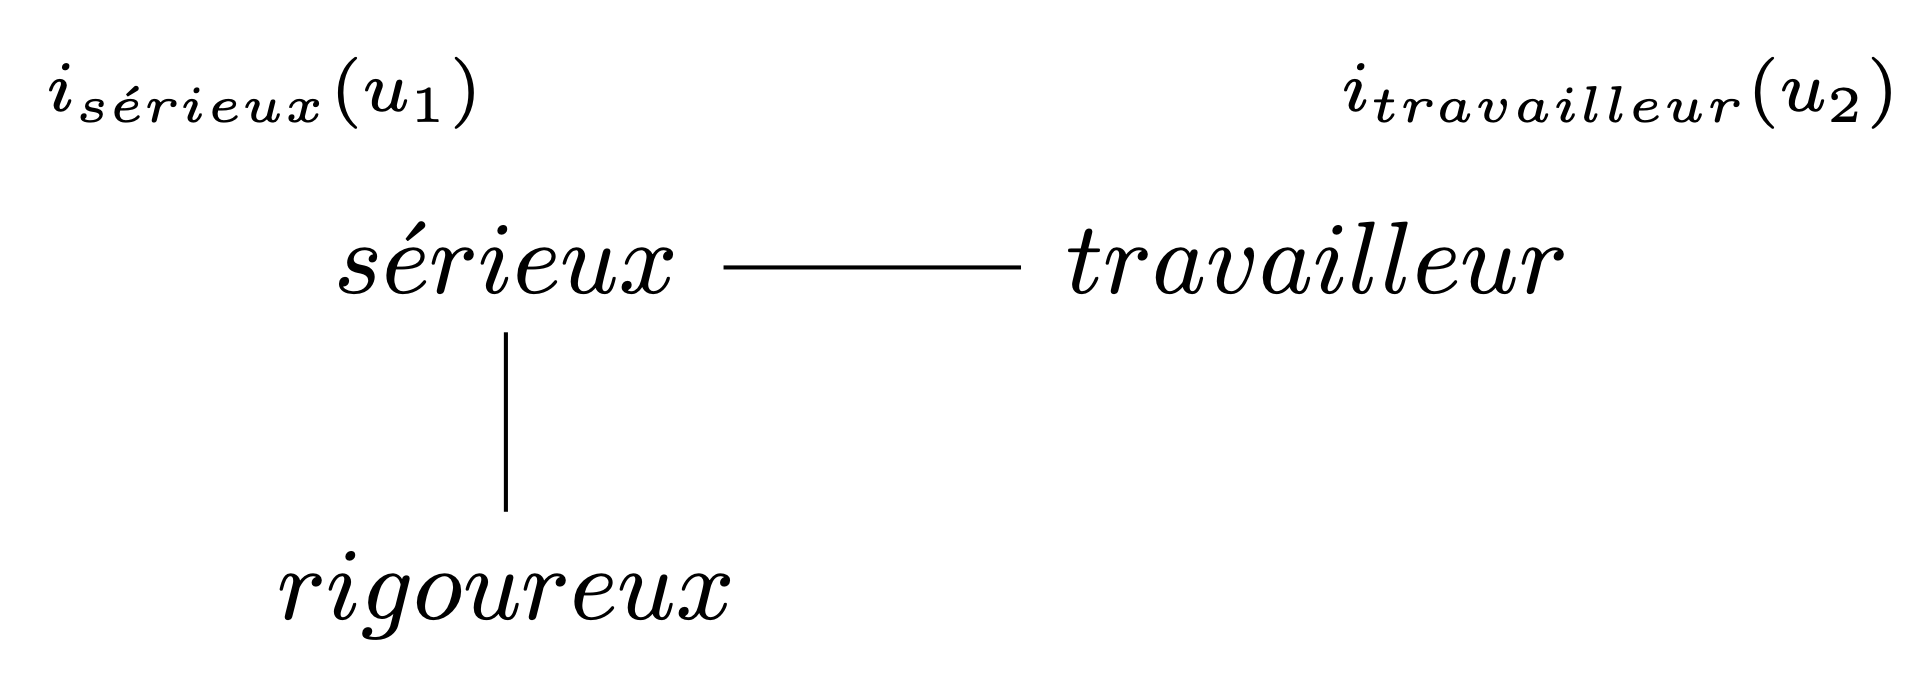
\includegraphics[scale=0.25]{Images/image_graphe_ex.png}
    \caption{Esquisse d'un sous graphe du graphe de proximité sémantique illustrant la proximité des concepts 'sérieux', 'travailleur' et 'rigoureux'. Ici, un utilisateur $u_1$ est sérieux avec intensité $i_{s\acute erieux}(u_1)$, et l'utilisateur $u_2$ est travailleur avec l'intensité $i_{travailleur}(u_2)$.}
    \label{fig:graphe schématique}
\end{figure}

Pour fixer les idées, proposons une telle distance $\Delta$ entre les utilisateurs $u_1$ et $u_2$, en supposant le graphe de proximité sémantique $G$ déjà construit. Pour cela, nous avons seulement besoin d'une distance sur $G\times\mathbb{R}$ notée $\delta$. A titre d'exemple, prenons
$$
\delta[(c,i),(c',i')]=dist_G(c,c')+|i-i'|,
$$
où $dist_G(c,c')$ est la longueur du plus court chemin reliant les concepts $c$ et $c'$ dans le graphe $G$. Pour un concept $c$ donné, la valeur $min_{c'\in G}\delta[(c,i_c(u_1)),(c',i_{c'}(u_2))]$ mesure alors l'affinité (unidirectionnelle) qu'éprouve $u_1$ à l'égard de $u_2$ au travers du concept $c$. Pour obtenir une mesure bidirectionnelle puis globale de l'affinité entre $u_1$ et $u_2$, il reste à calculer de même l'affinité de $u_2$ à l'égard de $u_1$ au travers de $c$, puis à sommer sur l'ensemble des concepts. Au bout du compte, on obtient la formule
$$
\Delta (u_1,u_2)=\sum_{c\in G}min_{c'\in G}\delta[(c,i_c(u_1)),(c',i_{c'}(u_2))]+min_{c'\in G}\delta[(c,i_{c}(u_2),(c',i_{c'}(u_1)))],
$$
qui fournit bien une distance sur l'ensemble des utilisateurs. Cela signifie, entre autres, que deux utilisateurs $u_1$ et $u_2$ ont le même profil si $\Delta(u_1,u_2)=0$, et réciproquement. Plus généralement, on pourra dire (ou plutôt décréter) que les profils des deux utilisateurs sont d'autant plus compatibles que $\Delta(u_1,u_2)$ est petite. Concluons en indiquant que le choix de cette distance, et tout particulièrement le choix de $\delta$, est tout à fait arbitraire. Il s'agira de l'ajuster en fonction des besoins et des attentes.

Dans le reste de ce travail, on se focalise uniquement sur la construction du graphe sous-jacent modélisant la proximité sémantique entre les différents concepts de la langue française. On ne parlera donc plus ni des utilisateurs, ni de leur réponse à un questionnaire, et encore moins de la façon par laquelle on pourrait établir automatiquement leur affinité avec tel ou tel concept.

\section{Construction du graphe de proximité sémantique}

Le graphe que l'on propose de construire est non dirigé, et deux sommets sont liés par une arête au plus. Il s'agit donc d'identifier les sommets du graphe puis de déterminer sous quelles conditions deux sommets seront liés par une arête. Il serait également appréciable de pouvoir affecter une pondération à chaque arête, afin de pouvoir quantifier le degré de proximité entre ces concepts. Dans tout ce projet, nous utilisons le langage de programmation Python.

\subsection{Identification des sommets}
Rappelons que les sommets du graphe que l'on cherche à construire ont vocation à modéliser les concepts inhérents à la langue française. Nous avons choisi de représenter un concept non par un mot, mais par une définition. En effet, à un même mot peuvent correspondre plusieurs définitions. Le plus souvent, c'est le contexte de l'usage d'un mot qui en détermine le sens. À l'inverse, deux mots exprimant le même concept ont des définitions proches.

Nous utilisons la bibliothèque NLTK \cite{loper2002nltk} et son module Wordnet \cite{fellbaum2010wordnet} pour récupérer les concepts et leur définition. L'utilisation de ces outils engendre cependant une difficulté, puisque les concepts et définitions ainsi obtenues sont exprimées en anglais. Nous utilisons la bibliothèque \verb|googletrans| pour obtenir un équivalent français.

\subsection{Identification des liens sémantiques}
Pour identifier les liens sémantiques entre deux concepts, c'est à dire entre deux définitions, nous procédons en deux étapes. Il convient tout d'abord d'encoder chaque définition en un vecteur afin d'interpréter le sens de cette phrase d'une manière numérique. Nous serons ensuite en mesure de développer une méthode pour mesurer la proximité sémantique entre deux concepts. 

\subsubsection{Interprétation numérique de la sémantique via une bibliothèque NLP}
Les bibliothèques NLP (Natural Language Processing ou Traitement Automatique du Langage Naturel en français) contextuelles sont conçues pour traiter et comprendre le langage dans des contextes variés. Nous utilisons le modèle CamemBERT \cite{martin-etal-2020-camembert, martin:hal-02784755}, spécifiquement pré-entraîné sur un corpus français. Il s'agit d'un réseau de neurones de type \textit{transformer} conçu pour modéliser les dépendances à longue portée dans les séquences de mots. A l'origine, CamemBERT a été développé en tant qu'IA générative, c'est-à-dire qu'il est capable, étant donné une phrase à trou, de retrouver le mot manquant le plus probable.

De façon interne, à partir d'une phrase fournie en entrée, CamemBERT génère une collection de vecteurs représentant la sémantique de la phrase. Plus précisément, CamemBERT segmente la phrase en unités appelées \textit{token}, qui sont à peu de chose près les mots de la phrases. Chaque unité est alors convertie en un vecteur représentant son sens, en prenant en compte le contexte dans lequel l'unité est rencontrée. En tant qu'IA générative, CamemBERT offre également la possibilité de positionner le mot-clef \verb|<mask>| au sein de la phrase d'entrée, indiquant ainsi la place d'un mot inconnu à deviner.

Dans le cadre de notre projet, l'outil CamemBERT se prête à plusieurs types d'utilisation. Nous avons choisi de nous en servir de la façon suivante. Pour chaque concept, nous fournissons à CamemBERT la définition du concept. Puis nous récupérons la liste de vecteurs générée de manière interne par CamemBERT et représentant de façon quantitative la sémantique du concept.

\subsubsection{Mesure de la proximité sémantique}
Nous utilisons la représentation vectorielle ainsi obtenue pour mesurer la proximité sémantique entre deux concepts. Cette représentation numérique consiste en une suite de vecteurs. Le premier vecteur renvoyé par CamemBERT code la sémantique de l'ensemble de la phrase de manière globale. Les autres vecteurs apportent des informations plus spécifiques. Pour obtenir une représentation globale du sens de la phrase, il est classique de considérer, outre le premier vecteur, la moyenne de tous les vecteurs de la suite. C'est cette dernière méthode que nous avons employée pour obtenir un unique vecteur représentant la sémantique de ce concept.

Pour mesurer la distance sémantique entre deux concepts, nous utilisons de manière classique la distance cosinus entre les vecteurs ainsi associés à chacun des concepts, et qui revoit un score de similarité compris entre $-1$ et $1$. Plus les concepts sont similaires, et plus le score est proche de $1$. A l'inverse, deux concepts sans rapport apparent auront un score de similarité proche de $-1$. Décider si deux concepts sont suffisamment proches sémantiquement revient à fixer un seuil inférieur sur leur score de similarité. Pour cela, nous évaluons la distance entre quelques concepts, et choisissons une valeur en dessous de laquelle nous jugeons négligeable la proximité sémantique entre deux concepts. Dans ce qui suit, le seuil a été fixé à $0,8$. Bien sûr, ce choix est tout à fait arbitraire et devra être calibrer afin de correspondre aux attentes.

\section{Résultats}
Nous testons notre méthode sur les concepts engendrés par les mots 'voiture' et 'orange', représentés en Figure \ref{fig:concepts}. Nous obtenons un graphe dont les deux composantes connexes sont respectivement données en Figure \ref{fig:graph1} et Figure \ref{fig:graph2}.

\begin{figure}[h]
    \centering
    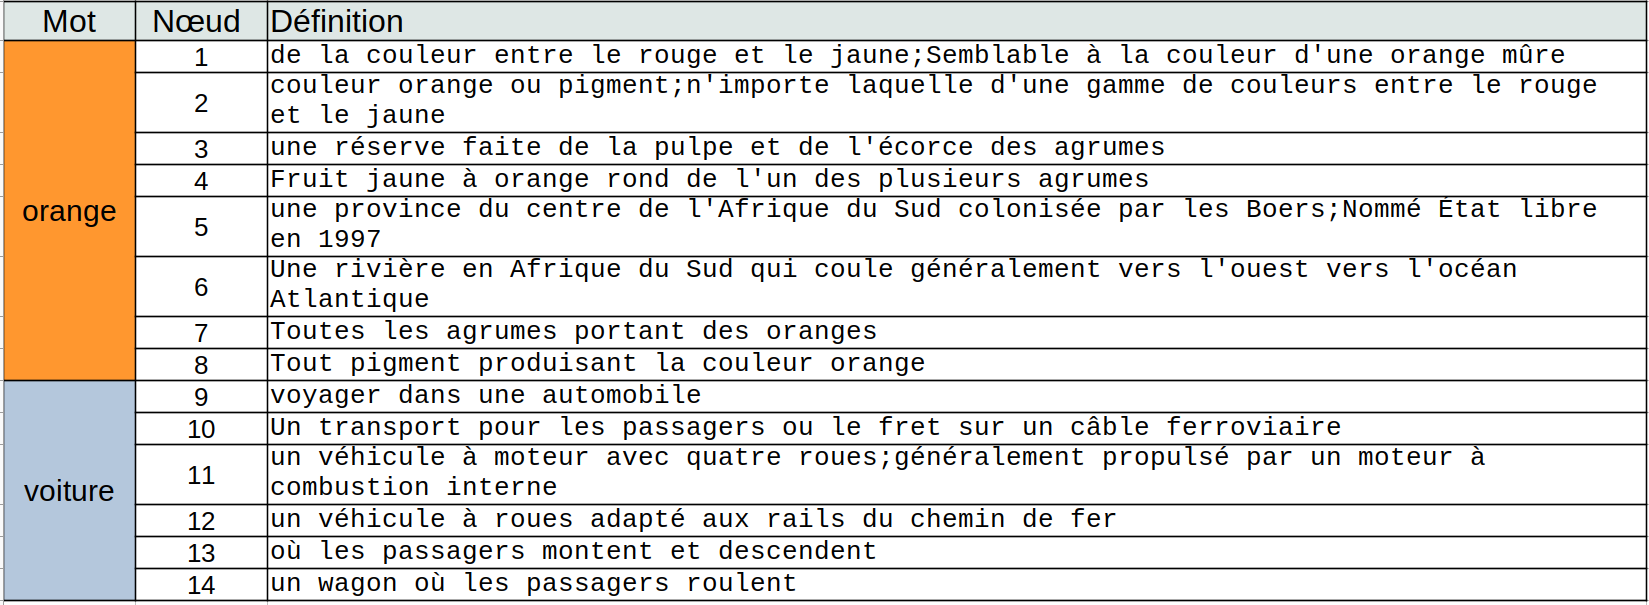
\includegraphics[scale=0.2]{Images/def_mot.png}
    \caption{Correspondance entre les concepts engendrés par les mots 'voiture' et 'orange', et les n\oe{}uds du graphe représenté en Figure \ref{fig:graph1} et Figure \ref{fig:graph2}. Le mot 'orange' possède 8 définitions et engendre ainsi 8 concepts. Le mot voiture possède 6 définitions, engendrant ainsi 6 concepts.}
    \label{fig:concepts}
\end{figure}

\begin{figure}[p]
    \centering
    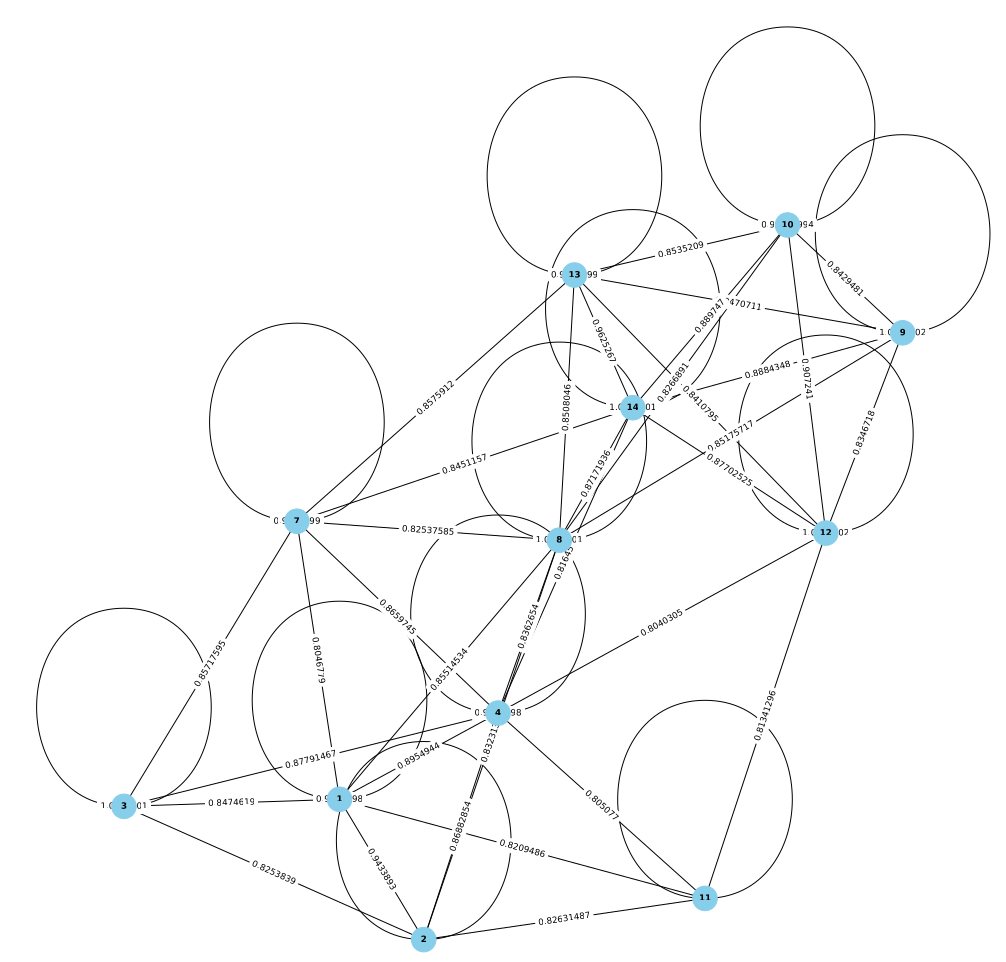
\includegraphics[scale=0.3]{Images/graphe_pt1.png}
    \caption{Composante connexe du graphe de proximité sémantique fournissant les liens sémantiques entre 12 des 14 concepts engendrés par les mots 'orange' et 'voiture'.}
    \label{fig:graph1}
\end{figure}

\begin{figure}[p]
    \centering
    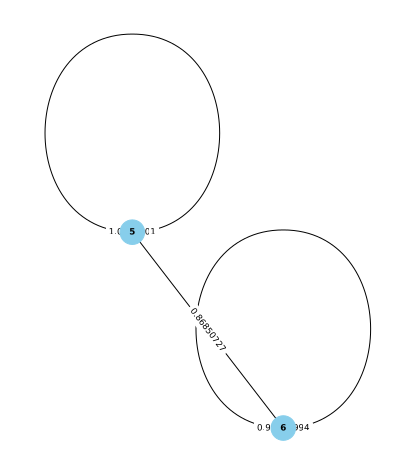
\includegraphics[scale=0.3]{Images/graphe_pt2.png}
    \caption{Composante connexe du graphe de proximité sémantique fournissant un lien sémantiques entre 2 des 14 concepts engendrés par les mots 'orange' et 'voiture'.}
    \label{fig:graph2}
\end{figure}

Il est intéressant de noter que la composante connexe de la Figure \ref{fig:graph2} regroupe les concepts $5$ et $6$ du tableau de la Figure \ref{fig:concepts}, qui sont deux notions liées à la géographie de l'Afrique du Sud, et qui ont en effet, selon le sens commun, peu de rapport avec le reste des concepts répertoriés en Figure \ref{fig:concepts}.

Le graphe présenté en Figure \ref{fig:graph1} et Figure \ref{fig:graph2} est pondéré. Nous avons effectivement choisi de conserver le score de similarité entre deux concepts et de l'affecter en tant que poids à l'arête reliant les deux concepts. Dans des applications futures, cette pondération pourra être utilisée, comme par exemple pour définir une distance sur $G$ autre que celle proposée en section \ref{sec:Identification du problème et objectifs}, en prenant en compte le degré de proximité sémantique entre les concepts.

Remarquons qu'il aurait tout à fait été possible de se passer du choix d'un seuil, et de construire un graphe complet (c'est-à-dire que tous les n\oe{}uds sont reliés deux à deux) pondéré par le score de similarité entre les n\oe{}uds. Cependant, d'une part les graphes complets sont gourmands en mémoire, et d'autre part leur représentation graphique est peu lisible. C'est pourquoi, dans le souci d'alléger le graphe final, nous avons décidé de ne pas conserver les arêtes les moins significatives en termes de proximité sémantique.

\section{Conclusion}

Cette étude a donc permis de développer une procédure de construction d'un graphe de proximité sémantique de la langue française et de tester cette procédure sur un cas simple. Néanmoins, la méthode que nous avons proposée n'est pas parfaite et présente des limites. Notamment, les points suivants posent des difficultés et pourraient être améliorés.

\begin{itemize}
    \item Le fait de passer par un traducteur ajoute du biais. Il faudrait utiliser un dictionnaire français \cite{sagot2008building, GLAWI}.
    \item Une étude doit être faite sur le choix du seuil concernant le score de similarité.
    \item Les concepts essentiels doivent être déterminés. En effet, beaucoup de mots, comme par exemples les déterminants, s'avèrent peu signifiants, et n'ont donc pas leur place dans un graphe sémantique. De plus, l'utilisation de toutes les définitions de tous les mots du dictionnaire risque de donner lieu à des redondances.
    \item Le calcul des représentations vectorielles est coûteux, et nécessite des ressources de calcul importantes.
    \item Le choix d'un vecteur pour représenter une définition doit être débattu. Nous nous sommes en effet concentré sur le premier vecteur et sur la moyenne des vecteurs de la liste générée par CamemBERT, mais d'autres choix seraient envisageables. Par exemple, nous pourrions choisir comme représentant la concaténation des vecteurs de la liste.
    \item La distance cosinus servant à mesurer le score de similarité entre deux concepts semble faire autorité dans le milieu des NLP, mais il serait intéressant d'étudier d'autres types de distances.
    \item Le choix des phrases utilisées en entrée de CamemBERT est à discuter dans l'optique d'améliorer les résulats. Par exemple, plutôt que de fournir à CamemBERT uniquement la définition $def$ d'un concept associé à un mot $mot$, il serait intéressant de construire la phrase \enquote{$mot:def$}, et d'utiliser cette phrase en entrée de CamemBERT. Nous pourrions également penser à préciser la nature grammaticale du mot, comme fréquemment indiqué dans les dictionnaires. Alternativement, la phrase \enquote{\texttt{<mask>}:\textit{def}} pourrait être fournie en entrée de CamemBERT, ce qui aurait pour conséquence d'attirer l'attention de CamemBERT sur le mot manquant, qui est précisément le concept auquel on s'intéresse.
    \item Nous pourrions obtenir des résultats plus précis en ré-entraînant CamemBERT à répondre plus spécifiquement à notre problématique (ce procédé est appelé \textit{fine-tunning}). Pour cela, on pourrait entraîner CamemBERT sur un corpus [concepts, définitions].
    \item Les liens entre les différents concepts ne sauraient se résumer à une proximité sémantique. D'autres liens doivent être étudiés et représentés afin d'enrichir le graphe.
\end{itemize}
\clearpage

% Bibliographie
% \section*{Références}
\printbibliography
    
\end{document}
